\documentclass[11pt, a4paper]{article}
\usepackage{graphicx}
\usepackage{amsmath}
\usepackage{listings}


\title{EE2703 Final Exam} % Title

\author{Harshavardhan Mudadla} % Author name

\date{\today} % Date for the report
\begin{document}		
		
\maketitle % Insert the title, author and date
\section{Pseudo Code for Question1}
%Create new section;it is autonumbered
We are trying to compute points to work on.\\
1. Divide the wire into pieces of length dz and so, we have $2N$ pieces and $2N+1$ points.\\
2. Then we are going to create an array "z" of length $2N+1$ which contains point coordinates.This is done using $"linspace"$ command.\\
3. We will take construct array of length $2N-2$ which will not have coordinates $-0.5,0,0.5$ was done by deleting it from z. 
4. We are going to compute at $N = 4$.

\subsection{Matrices Obtained}
\begin{lstlisting}	
Vector z :
    [-0.5  -0.38 -0.25 -0.12  0.    0.12  0.25  0.38  0.5]
Vector u :
    [-0.38 -0.25 -0.12  0.12  0.25  0.38]

\end{lstlisting}

\newpage
\section{Pseudo Code for Question2}
We need an equation for each unknown current. These equations are obtained by
calculating the Magnetic field in two different ways.\\
\\
From Ampere's Law:\\
\\
1. We have $H = M*J$.We will compute H at $r = a$\\
2. We will construct matrix M by using $"identity"$ command to get unit matrix of size $(2N-2,2N-2)$ 
\subsection{Matrices Obtained}
\begin{lstlisting}	
Matrix M:
   [[15.92  0.    0.    0.    0.    0.  ]
     [ 0.   15.92  0.    0.    0.    0.  ]
     [ 0.    0.   15.92  0.    0.    0.  ]
     [ 0.    0.    0.   15.92  0.    0.  ]
     [ 0.    0.    0.    0.   15.92  0.  ]
     [ 0.    0.    0.    0.    0.   15.92]]

\end{lstlisting}
\newpage
\section{Pseudo Code for Question3}
From Vector potential:\\
\\
1. We have to construct two Matrices $P and Pb$.\\
 P is the contribution to the vector potential due to currents unknown. It is a matrix with $2N−2$ columns and
$2N−2$ rows.\\
 Pb is the contribution to the vector potential due to current $z=0$. It is a column vector.\\
2. To construct those we are going to need $Rz, Ru, RiN$.\\
Rz computes distances including distances to known current.\\
 Ru is a vector of distances to unknown currents.\\
 RiN is distances with respect to z = 0 coordinate.\\
3. We will have $zi$ in which we store all the points present in z vector multiple times in different rows of order$2N+1$.We will do the same for $zi$, but we store it different coloumns. These matrices obtained using $Meshgrid$ command.\\
4. For $Rz$ we will get the distances using these $Zi and zj$.\\
5. Similarly we will take $ui and uj$ with all points in u vector to obtain $Ru$.$RiN$ is obtained by deleting $0,N,2N$ indexed elements of $Rz$ in $N+1 th$ coloumn\\
6. From $Ru and Rin$ we will get $P and Pb$.
\subsection{Matrices Obtained}
\begin{lstlisting}	
Matrix Rz :
[[0.01+0.j 0.13+0.j 0.25+0.j 0.38+0.j 0.5 +0.j 0.63+0.j
0.75+0.j 0.88+0.j 1.  +0.j]

 [0.13+0.j 0.01+0.j 0.13+0.j 0.25+0.j 0.38+0.j 0.5 +0.j
 0.63+0.j 0.75+0.j 0.88+0.j]
 
 [0.25+0.j 0.13+0.j 0.01+0.j 0.13+0.j 0.25+0.j 0.38+0.j 
 0.5 +0.j 0.63+0.j 0.75+0.j]
 
 [0.38+0.j 0.25+0.j 0.13+0.j 0.01+0.j 0.13+0.j 0.25+0.j 
 0.38+0.j 0.5 +0.j 0.63+0.j]
 
 [0.5 +0.j 0.38+0.j 0.25+0.j 0.13+0.j 0.01+0.j 0.13+0.j
 0.25+0.j 0.38+0.j 0.5 +0.j]
 
 [0.63+0.j 0.5 +0.j 0.38+0.j 0.25+0.j 0.13+0.j 0.01+0.j
 0.13+0.j 0.25+0.j 0.38+0.j]
 
 [0.75+0.j 0.63+0.j 0.5 +0.j 0.38+0.j 0.25+0.j 0.13+0.j
 0.01+0.j 0.13+0.j 0.25+0.j]
 
 [0.88+0.j 0.75+0.j 0.63+0.j 0.5 +0.j 0.38+0.j 0.25+0.j
 0.13+0.j 0.01+0.j 0.13+0.j]
 
 [1.  +0.j 0.88+0.j 0.75+0.j 0.63+0.j 0.5 +0.j 0.38+0.j
 0.25+0.j 0.13+0.j 0.01+0.j]]
 
Matrix Ru :
    [[0.01+0.j 0.13+0.j 0.25+0.j 0.5 +0.j 0.63+0.j 0.75+0.j]
     [0.13+0.j 0.01+0.j 0.13+0.j 0.38+0.j 0.5 +0.j 0.63+0.j]
     [0.25+0.j 0.13+0.j 0.01+0.j 0.25+0.j 0.38+0.j 0.5 +0.j]
     [0.5 +0.j 0.38+0.j 0.25+0.j 0.01+0.j 0.13+0.j 0.25+0.j]
     [0.63+0.j 0.5 +0.j 0.38+0.j 0.13+0.j 0.01+0.j 0.13+0.j]
     [0.75+0.j 0.63+0.j 0.5 +0.j 0.25+0.j 0.13+0.j 0.01+0.j]]
     
Vector RiN :
    [0.38+0.j 0.25+0.j 0.13+0.j 0.13+0.j 0.25+0.j 0.38+0.j]
    
Matrix P*1e8 : 
[[124.94-3.93j   9.2 -3.83j   3.53-3.53j  -0.  -2.5j
-0.77-1.85j -1.18-1.18j]

 [  9.2 -3.83j 124.94-3.93j   9.2 -3.83j   1.27-3.08j
 -0.  -2.5j -0.77-1.85j]
 
 [  3.53-3.53j   9.2 -3.83j 124.94-3.93j   3.53-3.53j
 1.27-3.08j -0.  -2.5j ]
 
 [ -0.  -2.5j    1.27-3.08j   3.53-3.53j 124.94-3.93j
 9.2 -3.83j 3.53-3.53j]
 
 [ -0.77-1.85j  -0.  -2.5j    1.27-3.08j   9.2 -3.83j
 124.94-3.93j 9.2 -3.83j]
 
 [ -1.18-1.18j  -0.77-1.85j  -0.  -2.5j    3.53-3.53j
 9.2 -3.83j 124.94-3.93j]]
 
Vector Pb*1e8:
    [1.27-3.08j 3.53-3.53j 9.2 -3.83j 9.2 -3.83j 3.53-3.53j 1.27-3.08j]

\end{lstlisting}
\newpage

\section{Pseudo Code for Question4}
1. We have to construct two Matrices $Q and Qb$.\\
 Q is the contribution due to currents unknown. It is a matrix with $2N−2$ columns and
$2N−2$ rows.\\
 Pb is the contribution due to current at $z=0$. It is a column vector.\\
2. To construct those we are going to need $Rz, Ru, RiN$.\\
3. From $Ru and Rin$ we will get $Q and Qb$.

\subsection{Matrices Obtained}
\begin{lstlisting}	
Matrix Q :
[[9.952e+01-0.j 5.000e-02-0.j 1.000e-02-0.j 0.000e+00-0.j 0.000e+00-0.j
  0.000e+00-0.j]
 [5.000e-02-0.j 9.952e+01-0.j 5.000e-02-0.j 0.000e+00-0.j 0.000e+00-0.j
  0.000e+00-0.j]
 [1.000e-02-0.j 5.000e-02-0.j 9.952e+01-0.j 1.000e-02-0.j 0.000e+00-0.j
  0.000e+00-0.j]
 [0.000e+00-0.j 0.000e+00-0.j 1.000e-02-0.j 9.952e+01-0.j 5.000e-02-0.j
  1.000e-02-0.j]
 [0.000e+00-0.j 0.000e+00-0.j 0.000e+00-0.j 5.000e-02-0.j 9.952e+01-0.j
  5.000e-02-0.j]
 [0.000e+00-0.j 0.000e+00-0.j 0.000e+00-0.j 1.000e-02-0.j 5.000e-02-0.j
  9.952e+01-0.j]]
  
Matrix Qb :
[0.  -0.j 0.01-0.j 0.05-0.j 0.05-0.j 0.01-0.j 0.  -0.j]

\end{lstlisting}
\newpage

\section{Pseudo Code for Question5}
1. Our final equation is $M*J = Q*J +QbIm$\\
i.e.,$(M −Q)*J = Qb*Im$\\
2. We will use $"inv(M-Q)$ to solve for $J$.\\
3. We construct the another vector with known currents and unknown currents.


\\
\\
We will get the exact curves on increasing N value.
\subsection{Matrices Obtained}
\begin{lstlisting}	
Icalculated :
[0. 0. 0. 0. 1. 0. 0. 0. 0.]

Iassumed :
[0.   0.38 0.71 0.92 1.   0.92 0.71 0.38 0.  ]

\end{lstlisting}

\subsection{Plots}
\begin{figure}[!tbh]
   	\centering
   	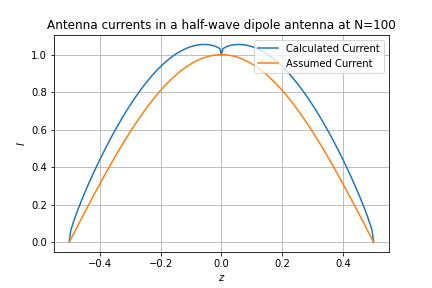
\includegraphics[scale=0.6]{fig1.png}  % Mention the image name within the curly braces. Image should be in the same folder as the tex file. 
   	\caption{Antenna currents in a half-wave dipole antenna at N=10}
   	\label{fig:sample}
   \end{figure}
   
   \begin{figure}[!tbh]
   	\centering
   	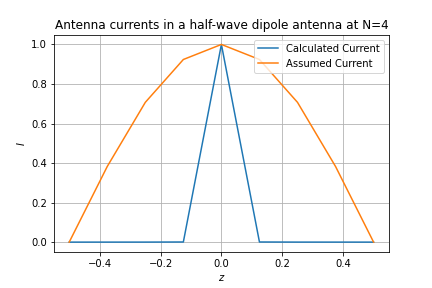
\includegraphics[scale=0.6]{fig2.png}  % Mention the image name within the curly braces. Image should be in the same folder as the tex file. 
   	\caption{Antenna currents in a half-wave dipole antenna at N=4}
   	\label{fig:sample}
   \end{figure}
\end{document}
